\chapter{Transaction Tracing}

Here we present a model of transaction tracing in Alloy, based on the OCF. The model is a stylized version of the OCF, and it is not intended to be a complete model of the OCF.

In this chapter, we choose to reduce the transaction system do its essential form\cite{DJSALLA}. The key abstraction in the transaction system is that of \textit{securities} which under go \textit{transactions}. 

In the original model, transactions take input securities and have output securities. Although there is a large number of different specialized transactions in the model, having Issuances, Cancellations and Transfers is enough to find the deep abstraction that allows securities to be traced to their original creation event (using Alloy), and thus form a history of a security including its lineage of parent securities.

One key problem in this is that writing a bunch of abstractions and then merging them in an actual programming language seldom works\cite{DJSALLA}. The reason, according to Daniel Jackson, is that:

\begin{quotation}
	The environment of programming is so much more exacting than the environment of sketching design abstractions. The compiler admits no vagueness whatsoever.\cite{DJSALLA}
\end{quotation}

Alloy can readily provide a visualization of what is called the meta-model (Alloy's representation of the model). 

\noindent\todo{Give a more precise description of the relationship between model and meta-model in Alloy}

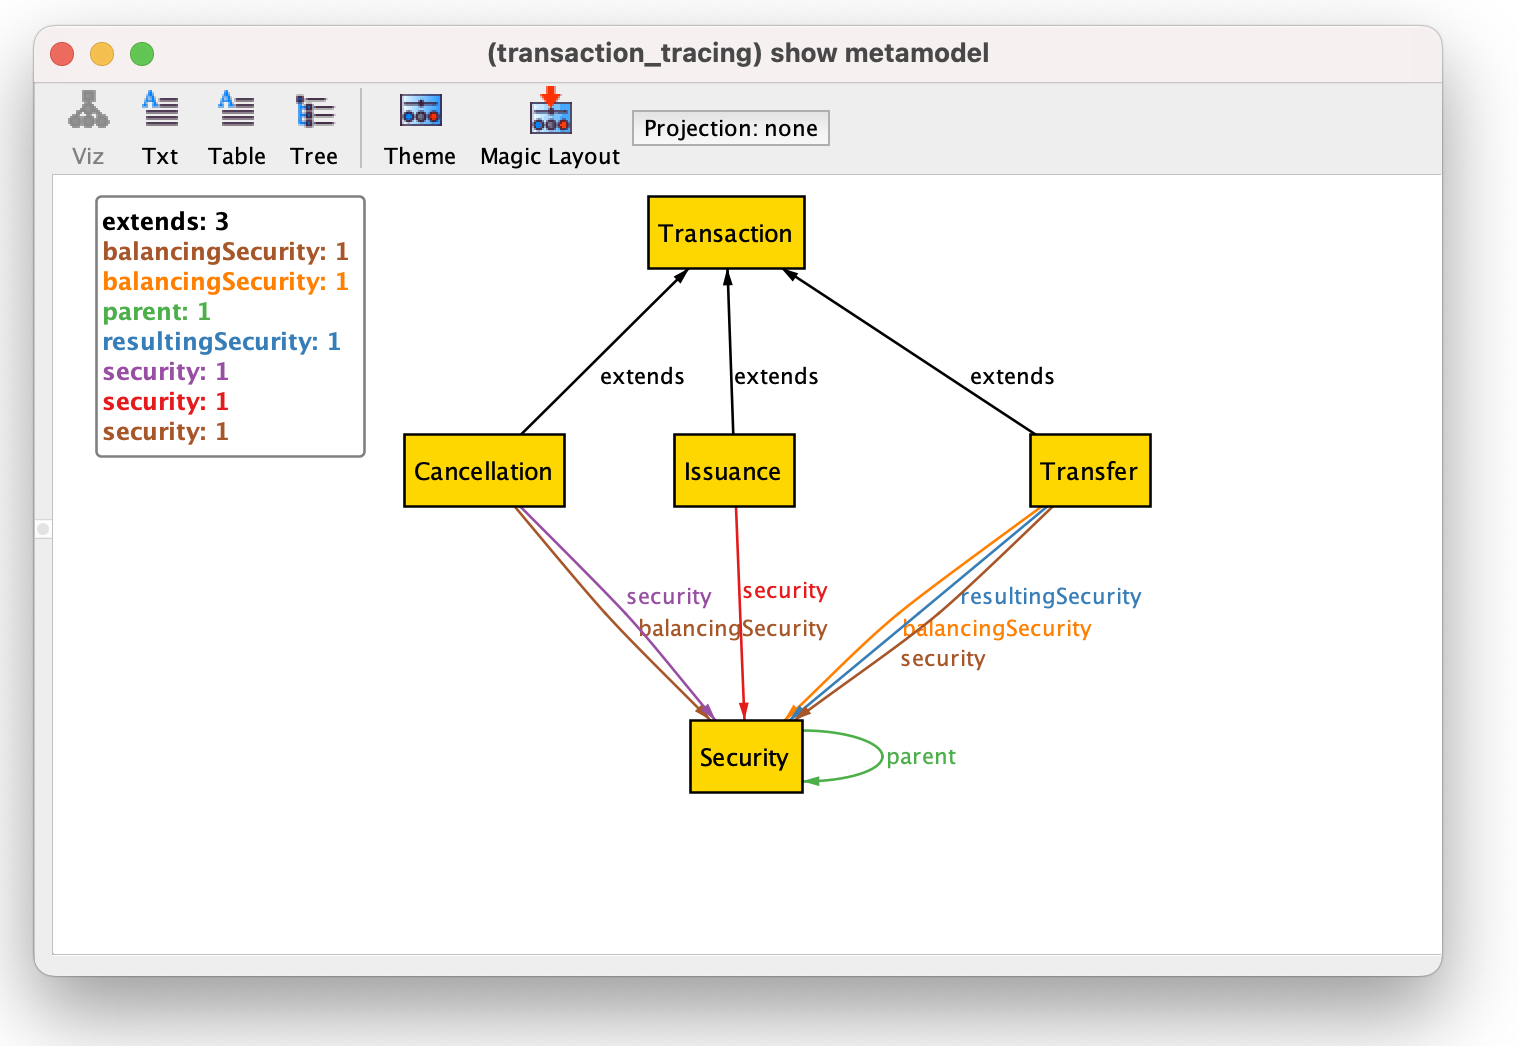
\includegraphics[width=0.8\textwidth]{pics/stock-transaction-tracing.png}

% SECTION: Signatures
\section{Signatures}

% SUBSECTION: The Security
\subsection{The Security}

\begin{listing}[!h]
\begin{minted}{alloy}
sig Security {
    shares : one Int,
    parent : lone Security
}
\end{minted}
\caption{The Security signature}
\label{lst:security-sig-1}
\end{listing}


The \texttt{Security} signature represents a security and includes the number of shares (\texttt{shares}) and a reference to its parent security (\texttt{parent}).

% SUBSECTION: The Abstract Transaction
\subsection{The Abstract Transaction}

\begin{listing}[!h]
\begin{minted}{alloy}
	abstract sig Transaction {}
\end{minted}
\caption{The Abstract Transaction signature}
\label{lst:transaction-sig-1}
\end{listing}

The \texttt{Transaction} signature is an abstract signature representing a transaction.

% SUBSECTION: The Issuance
\subsection{The Issuance}
\begin{listing}[!h]
\begin{minted}{alloy}
	sig Issuance extends Transaction {
		security : one Security,
		amount : one Int
	}
\end{minted}
\caption{The Issuance signature}
\label{lst:issuance-sig-1}
\end{listing}

The \texttt{Issuance} signature represents an issuance transaction, which creates a security with a specified amount of shares.

% SUBSECTION: The Cancellation
\subsection{The Cancellation}
\begin{listing}[!h]
\begin{minted}{alloy}
	sig Cancellation extends Transaction {
		security : one Security,
		amount : one Int,
		balancingSecurity : lone Security
	}
\end{minted}
\caption{The Cancellation signature}
\label{lst:cancellation-sig-1}
\end{listing}

The \texttt{Cancellation} signature represents a cancellation transaction, which destroys a certain amount of shares from a security. In case of a partial cancellation, a \texttt{balancingSecurity} is created to balance the number of shares.

% SUBSECTION: The Transfer
\subsection{The Transfer}
\begin{listing}[!h]
\begin{minted}{alloy}
	sig Transfer extends Transaction {
		security : one Security,
		amount : one Int,
		from : one Stakeholder,
		to : one Stakeholder,
		balancingSecurity : lone Security,
		resultingSecurity : one Security
	}
\end{minted}
\caption{The Transfer signature}
\label{lst:transfer-sig-1}
\end{listing}

The \texttt{Transfer} signature represents a transfer transaction, which moves a certain amount of shares from one stakeholder to another. If the transfer is partial, a \texttt{balancingSecurity} is created to balance the number of shares, and a \texttt{resultingSecurity} represents the resulting security after the transfer.

% Abstract sig Stakeholder {}
\subsection{The Stakeholder}
\begin{listing}[!h]
\begin{minted}{alloy}
	abstract sig Stakeholder {}
\end{minted}
\caption{The Stakeholder signature}
\label{lst:stakeholder-sig-1}
\end{listing}

The \texttt{Stakeholder} signature is an abstract signature representing a stakeholder.

% SECTION: Constraints
\section{Constraints}

% SUBSECTION: Requiring that all securities are created by an issuance
\subsection{Requiring that all securities are created by an issuance}
\begin{listing}[!h]
\begin{minted}{alloy}
	fact giveIssuanceToBalancingSecurity {
		all c : Cancellation | some c.balancingSecurity implies one i : Issuance | i.security = c.security
	}
	
	fact giveIssuanceToResultingSecurity {
		all t : Transfer | one i : Issuance | i.security = t.resultingSecurity
	}
\end{minted}
\caption{Requiring that all securities are created by an issuance}
\label{lst:issuance-constraint-1}
\end{listing}

These constraints ensure that every security involved in a cancellation or transfer is created by an issuance.

% SUBSECTION: Avoiding cycles
\subsection{Avoiding cycles}
\begin{listing}[!h]
\begin{minted}{alloy}
	fact noSelfParent {
		no s : Security | s in s.^parent
	}
\end{minted}
\caption{Avoiding cycles}
\label{lst:no-self-parent-constraint-1}
\end{listing}

This constraint ensures that there are no cycles in the parent-child relationship of securities.

% SUBSECTION: Constraining the parent-child relationship
\subsection{Constraining the parent-child relationship}
\begin{listing}[!h]
\begin{minted}{alloy}
	fact establishParent {
		all t : Transfer | some t.balancingSecurity => t.balancingSecurity.parent = t.security
		all t : Transfer | t.resultingSecurity.parent = t.security
		all i : Issuance | no i.security.parent
		all c : Cancellation | some c.balancingSecurity => c.balancingSecurity.parent = c.security
	}
\end{minted}
\caption{Constraining the parent-child relationship}
\label{lst:establish-parent-constraint-1}
\end{listing}

These constraints establish the parent-child relationship between securities and their balancing securities, ensuring that the model is prepared for tracing.

% SUBSECTION: Giving meaningful values to amounts
\subsection{Giving meaningful values to amounts}
\begin{listing}[!h]
\begin{minted}{alloy}
	fact issuancesAlwaysPositive {
		all i : Issuance | pos[i.amount]
		all c : Cancellation | pos[c.amount]
		all t : Transfer | pos[t.amount]
	}
\end{minted}
\caption{Giving meaningful values to amounts}
\label{lst:amounts-constraint-1}
\end{listing}

These constraints enforce that the amounts in issuances, cancellations, and transfers are always positive.

% SUBSECTION: Balancing the number of shares
\subsection{Balancing the number of shares}
\begin{listing}[!h]
\begin{minted}{alloy}
	fact cancellationBalances {
		all c : Cancellation
		| some c.balancingSecurity <=> add[c.balancingSecurity.shares, c.amount] = c.security.shares
		
		all c : Cancellation
		| no c.balancingSecurity <=> c.amount = c.security.shares
	}
	
	fact issuanceBalances {
		all i : Issuance | i.security.shares = i.amount
	}
\end{minted}
\caption{Balancing the number of shares}
\label{lst:balances-constraint-1}
\end{listing}

These constraints ensure that the number of shares is balanced in cancellations and issuances.

% SECTION: Funs, or queries
\section{Funs, or queries}
\begin{listing}[!h]
\begin{minted}{alloy}
	fun history[s : Security] : set Transaction {
		s.*parent
	}
\end{minted}
\caption{The \texttt{history} fun}
\label{lst:history-fun-1}
\end{listing}

The \texttt{history} function returns the set of transactions that form the history of a given security.

% SECTION: Examples
\section{Examples}

\begin{listing}[!h]
\begin{minted}{alloy}
e1 : run {
    some Cancellation
}
\end{minted}
\caption{Example 1}
\label{lst:example-1}
\end{listing}


\begin{figure}[ht]
\centering
\caption{An example of a cancellation transaction}
\label{fig:transaction-tracing-for-stocks-example-1}
\end{figure}

\begin{listing}[!h]
\begin{minted}{alloy}
	e2 : run {
		some Transfer
	}
\end{minted}
\caption{Example 2}
\label{lst:example-2}
\end{listing}


\begin{figure}[ht]
\centering
	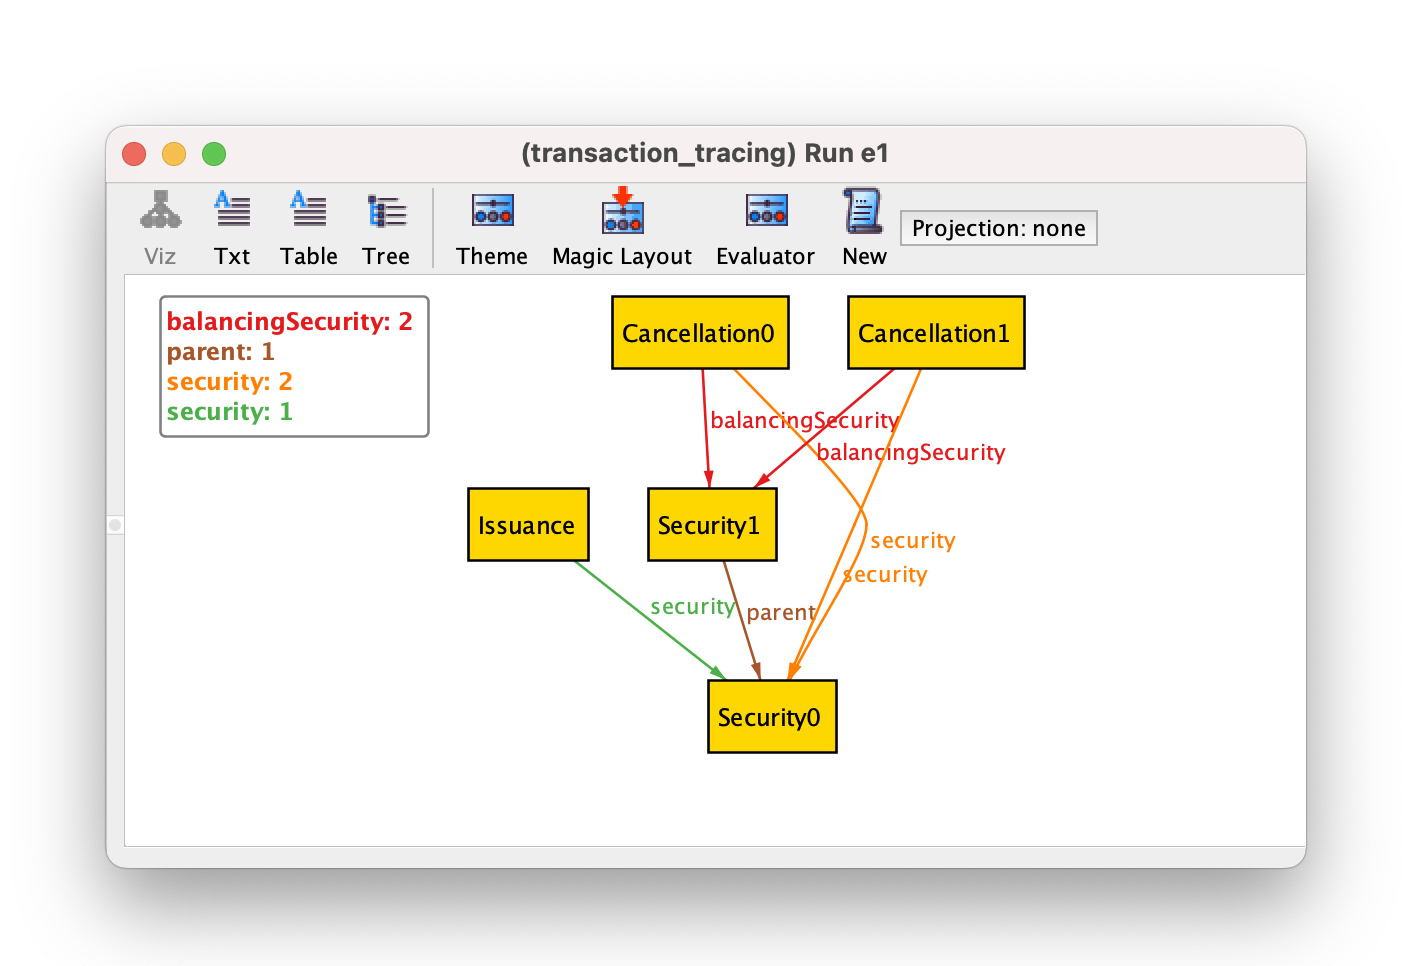
\includegraphics[width=0.8\textwidth]{pics/cancellation.png}
\caption{An example of a transfer transaction}
\label{fig:transaction-tracing-for-stocks-example-2}
\end{figure}

\begin{listing}[!h]
\begin{minted}{alloy}
e3 : run { some Issuance }
\end{minted}
\caption{Example 3}
\label{lst:example-3}
\end{listing}


\begin{figure}[ht]
\centering
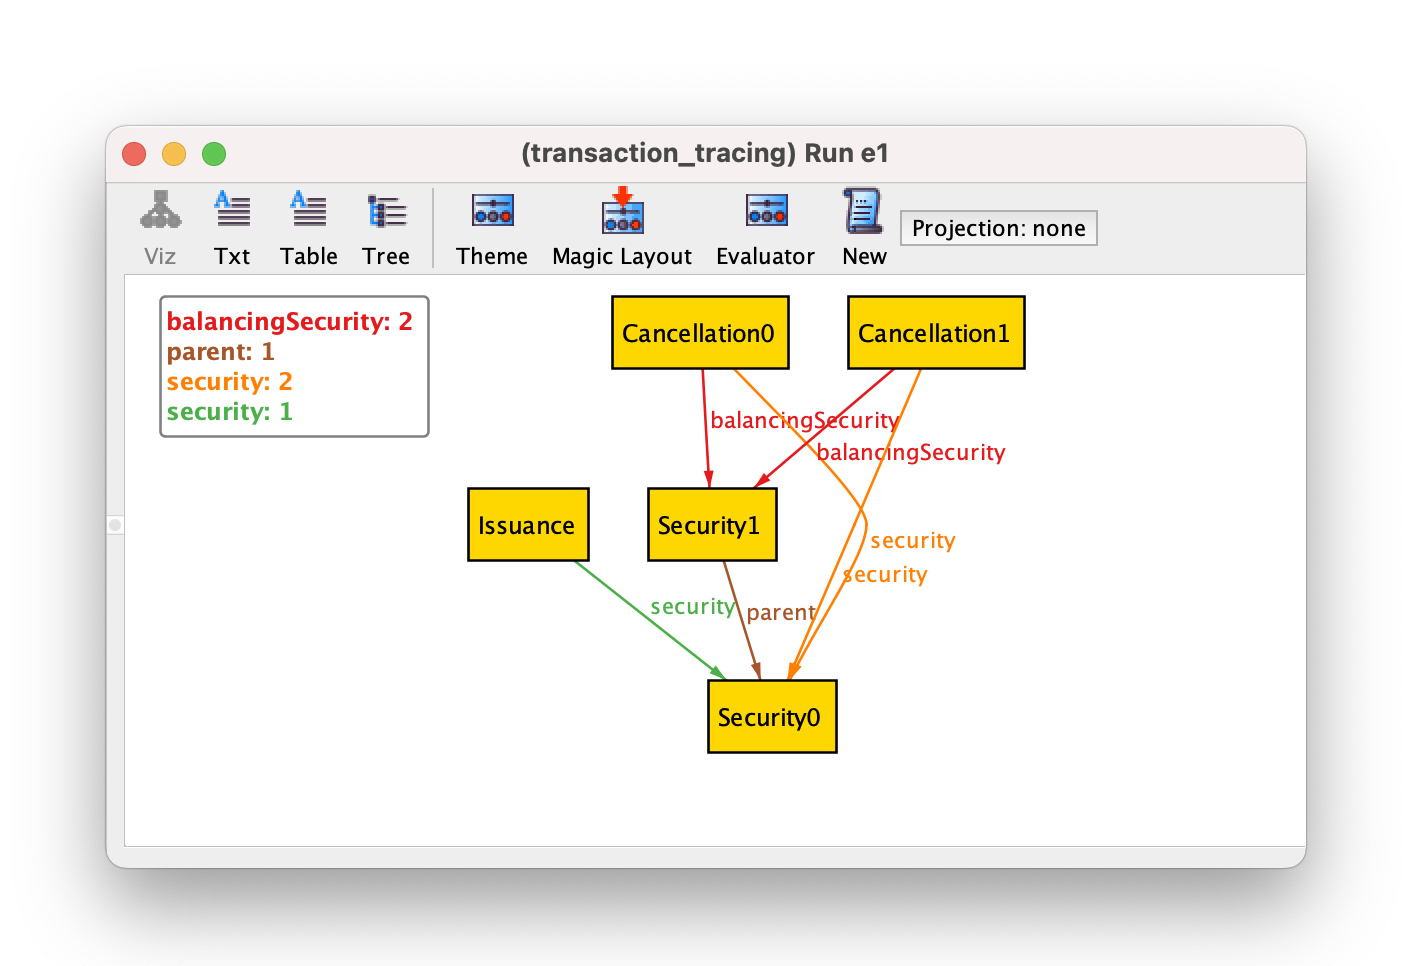
\includegraphics[width=0.8\textwidth]{pics/cancellation.png}
\caption{An example of an issuance transaction}
\label{fig:transaction-tracing-for-stocks-example-3}
\end{figure}

These examples demonstrate the usage of the model by running certain queries.

As a last example, we show how the improved model can picture long sequences of transactions, implied by many partial cancellations and transfers:

\begin{figure}
\centering
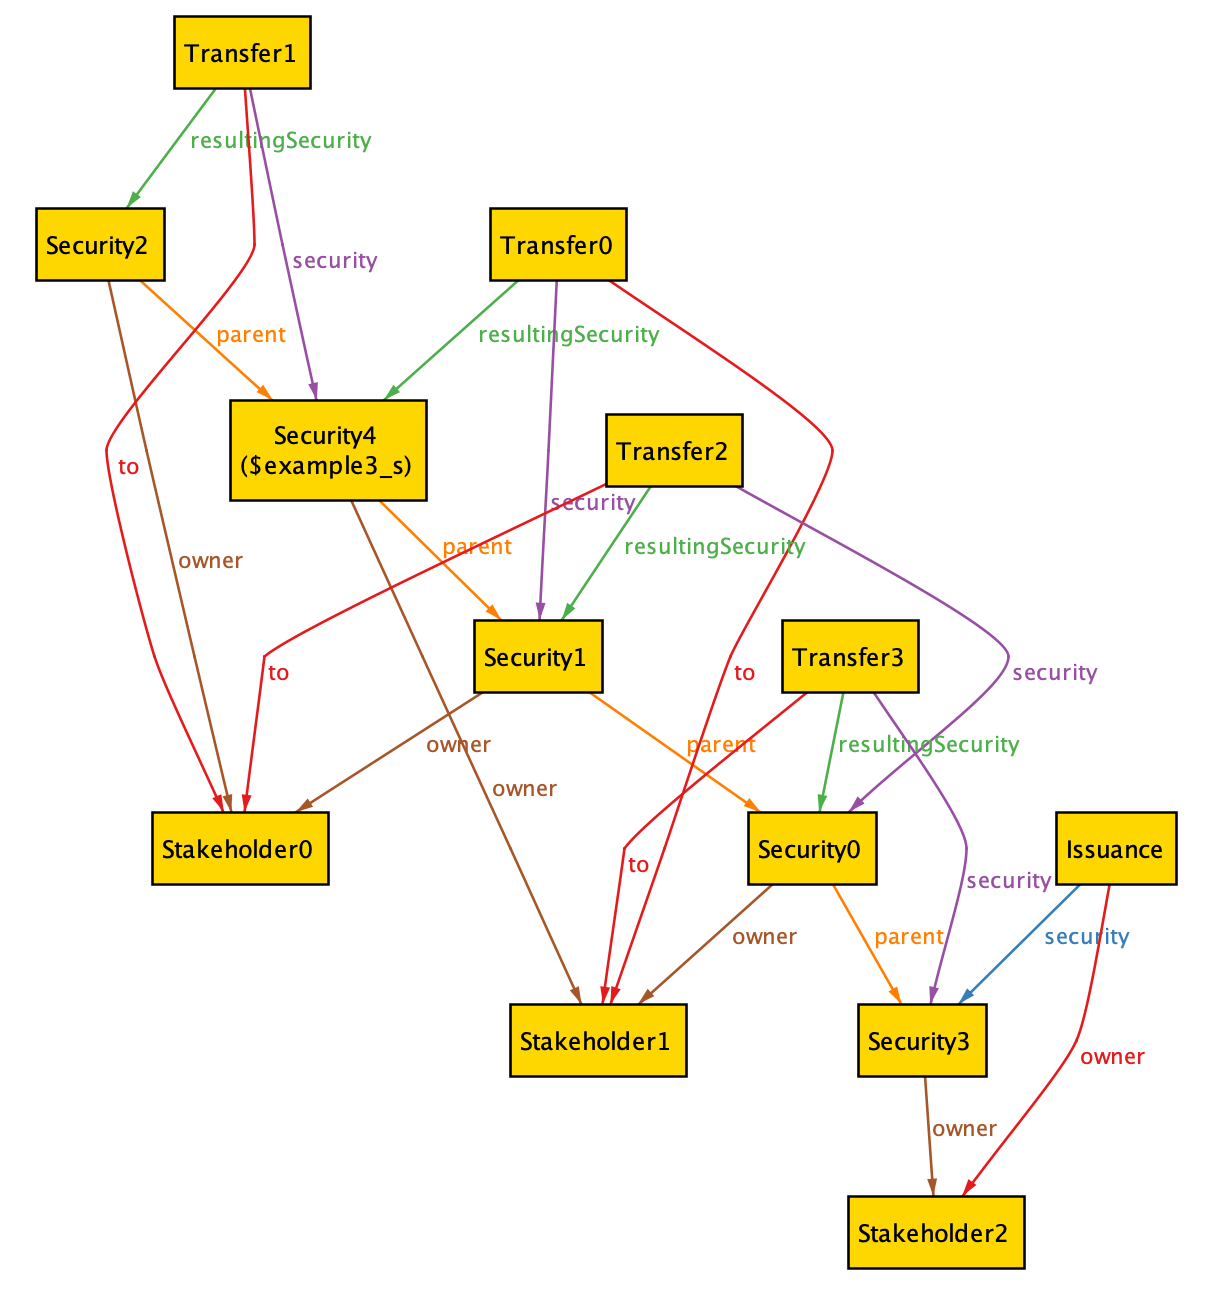
\includegraphics[width=0.8\textwidth]{pics/long-example.png}
\caption{An example of a long chain of transactions}
\label{fig:transaction-long-chain}
\end{figure}

% SECTION: Discussion
\section{Discussion}

By introducing a parent relationship to the security model, we were able to use Alloy's relational semantics to constrain the whole transitive closure of the parent relationship. This allowed us to model transaction tracing in a very robust way.

Furthermore, the constraints over the specific transaction types are required to validate them, and would not be possible in JSON Schema.

The translation was straightforward by declaring signatures and proceeding to constrain the signatures and relations based on the expected behavior of each transaction, according to the domain that is under consideration.

Checking the model was fast and brought solid confidence in the correctness of the model, by ruling out large classes of invalid models. We can point out that by choosing a size of 3 for the scope, we are considering a dizzying number of possible models\footnote{Certainly beyond the coverage provided by unit tests}, and yet the model checker was able to rule out all invalid models in a matter of seconds.

